\documentclass[letterpaper,11pt]{article}
\oddsidemargin -1.0cm \textwidth 17.5cm

\usepackage[utf8]{inputenc}
\usepackage[activeacute,spanish]{babel}
\usepackage{amsfonts,setspace}
\usepackage{amsmath}
\usepackage{amssymb, amsmath, amsthm}
\usepackage{comment}
\usepackage{amssymb}
\usepackage{dsfont}
\usepackage{anysize}
\usepackage{multicol}
\usepackage{enumerate}
\usepackage{graphicx}
\usepackage[left=1.5cm,top=2cm,right=1.5cm, bottom=1.7cm]{geometry}
\setlength\headheight{1.5em} 
\usepackage{fancyhdr}
\usepackage{multicol}
\usepackage{hyperref}
\usepackage{wrapfig}
\pagestyle{fancy}
\fancyhf{}
\renewcommand{\labelenumi}{\normalsize\bfseries P\arabic{enumi}.}
\renewcommand{\labelenumii}{\normalsize\bfseries (\alph{enumii})}
\renewcommand{\labelenumiii}{\normalsize\bfseries \roman{enumiii})}

\begin{document}

\fancyhead[L]{\itshape{Facultad de Ciencias F\'isicas y Matem\'aticas}}
\fancyhead[R]{\itshape{Universidad de Chile}}

\begin{minipage}{11.5cm}
    \begin{flushleft}
        \hspace*{-0.6cm}\textbf{FI1000-5 Introducción a la Física Clásica}\\
        \hspace*{-0.6cm}\textbf{Profesora:} Paulina Lira\\
        \hspace*{-0.6cm}\textbf{Auxiliares:} Alejandro Silva, Juan Cristobal Castro\\
    \end{flushleft}
\end{minipage}

\begin{picture}(2,3)
    \put(405,-5){
\includegraphics[scale=1.25]{2020-1/Imágenes/logo/fcfm2.pdf}}
\end{picture}

\begin{center}
	\LARGE \bf Auxiliar \#3: Caída libre y lanzamiento de proyectil   \\
\end{center}

\vspace{-1cm}
\begin{enumerate}\setlength{\itemsep}{0.4cm}

\rfoot[]{pág. \thepage}

\item[]

\item Si lanzo un objeto hacia arriba, desde el techo del costanera center, ubicado a 300 metros de altura con respecto al suelo, con una velocidad inicial $v_0$ = 35 m/s, ¿En cuanto tiempo llegaría ese objeto al suelo si consideramos condiciones ideales? (vacío) ¿Y si estuviéramos en la luna?\\
\textit{Hint: La gravedad en la luna es 1,62 m/s$^2$}

\begin{figure}[h!]
        \centering
        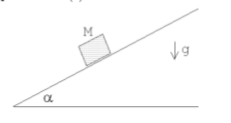
\includegraphics[scale=0.8]{../Imágenes/aux3/p1.png}
    \end{figure}


\item Un avión con cajas llenas de mascarillas e insumos médicos se mueve con extrema confidencialidad a lo largo de Chile repartiendo estos implementos, lo hace bajo tal nivel de secreto, que no puede aterrizar y solamente lanza los paquetes correspondientes a cada hospital desde la altura h a la que vuela. Si el avión vuela a una altura de 1500 m sobre el nivel del suelo y con una velocidad vo=360 km/hrs. ¿A que distancia horizontal L, con respecto al centro asistencial, debería lanzar los paquetes el avión?
    
   \begin{figure}[h!]
        \centering
        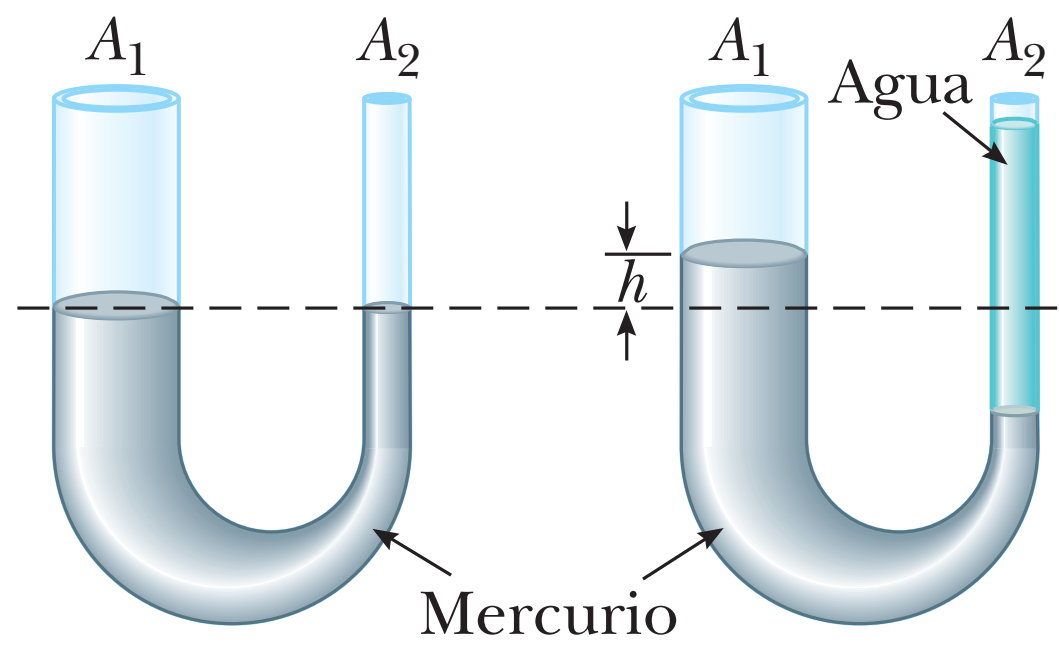
\includegraphics[scale=0.8]{../Imágenes/aux3/p2.png}
    \end{figure} 
    
\newpage
    
\item  En presencia de la gravedad terrestre una pelota saltarina entra con rapidez Vo por el techo de un pasillo de altura h. El ángulo de entrada de la pelota con respecto a la vertical es 
$\beta$ y y tanto el techo como el piso del pasillo son lisos y horizontales. La pelota rebota elástica e indefinidamente entre el piso y el techo.\\

a) Calcule el periodo T entre dos impactos consecutivos en el piso.\\
        
b) En ausencia de gravedad, calcule el periodo T entre dos impactos consecutivos en el piso. Verifique que este es un caso particular de su respuesta (a) \\

c) ¿Que distancia horizontal recorre la pelota entre dos impactos consecutivos con el suelo? (propuesto) \\
    
      \begin{figure}[h!]
        \centering
        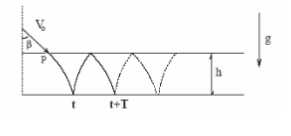
\includegraphics[scale=0.8]{../Imágenes/aux3/p3.png}
    \end{figure} 
    
       \begin{figure}[h!]
        \centering
        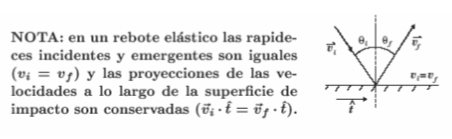
\includegraphics[scale=0.8]{../Imágenes/aux3/nota.png}
    \end{figure} 


\end{enumerate}
\end{document}